\subsection{研究内容}\label{ch2content}

本项目面向医疗卫生行业的数据分析需求,针对电子医疗记录分析存在的研究队列识别困
难、记录时间不规则、模型解释匮乏等问题,以深度学习为基础手段,研究电子医疗记录分
析建模的理论和方法,力争构建端到端的电子医疗记录分析方案,突破队列识别、EMR插补
和可解释性分析模型等关键技术,并在基于电子医疗记录的临床任务上验证本项目的研究成
果。

项目研究工作从队列识别、EMR插补、可解释分析模型和临床任务验证四个层次展开,本项
目的挑战、科学问题和研究内容关系如图~\ref{fig:ch2:rc}所示。各部分研究内容具体介
绍如下:

\begin{figure}
    \begin{small}
        \begin{center}
            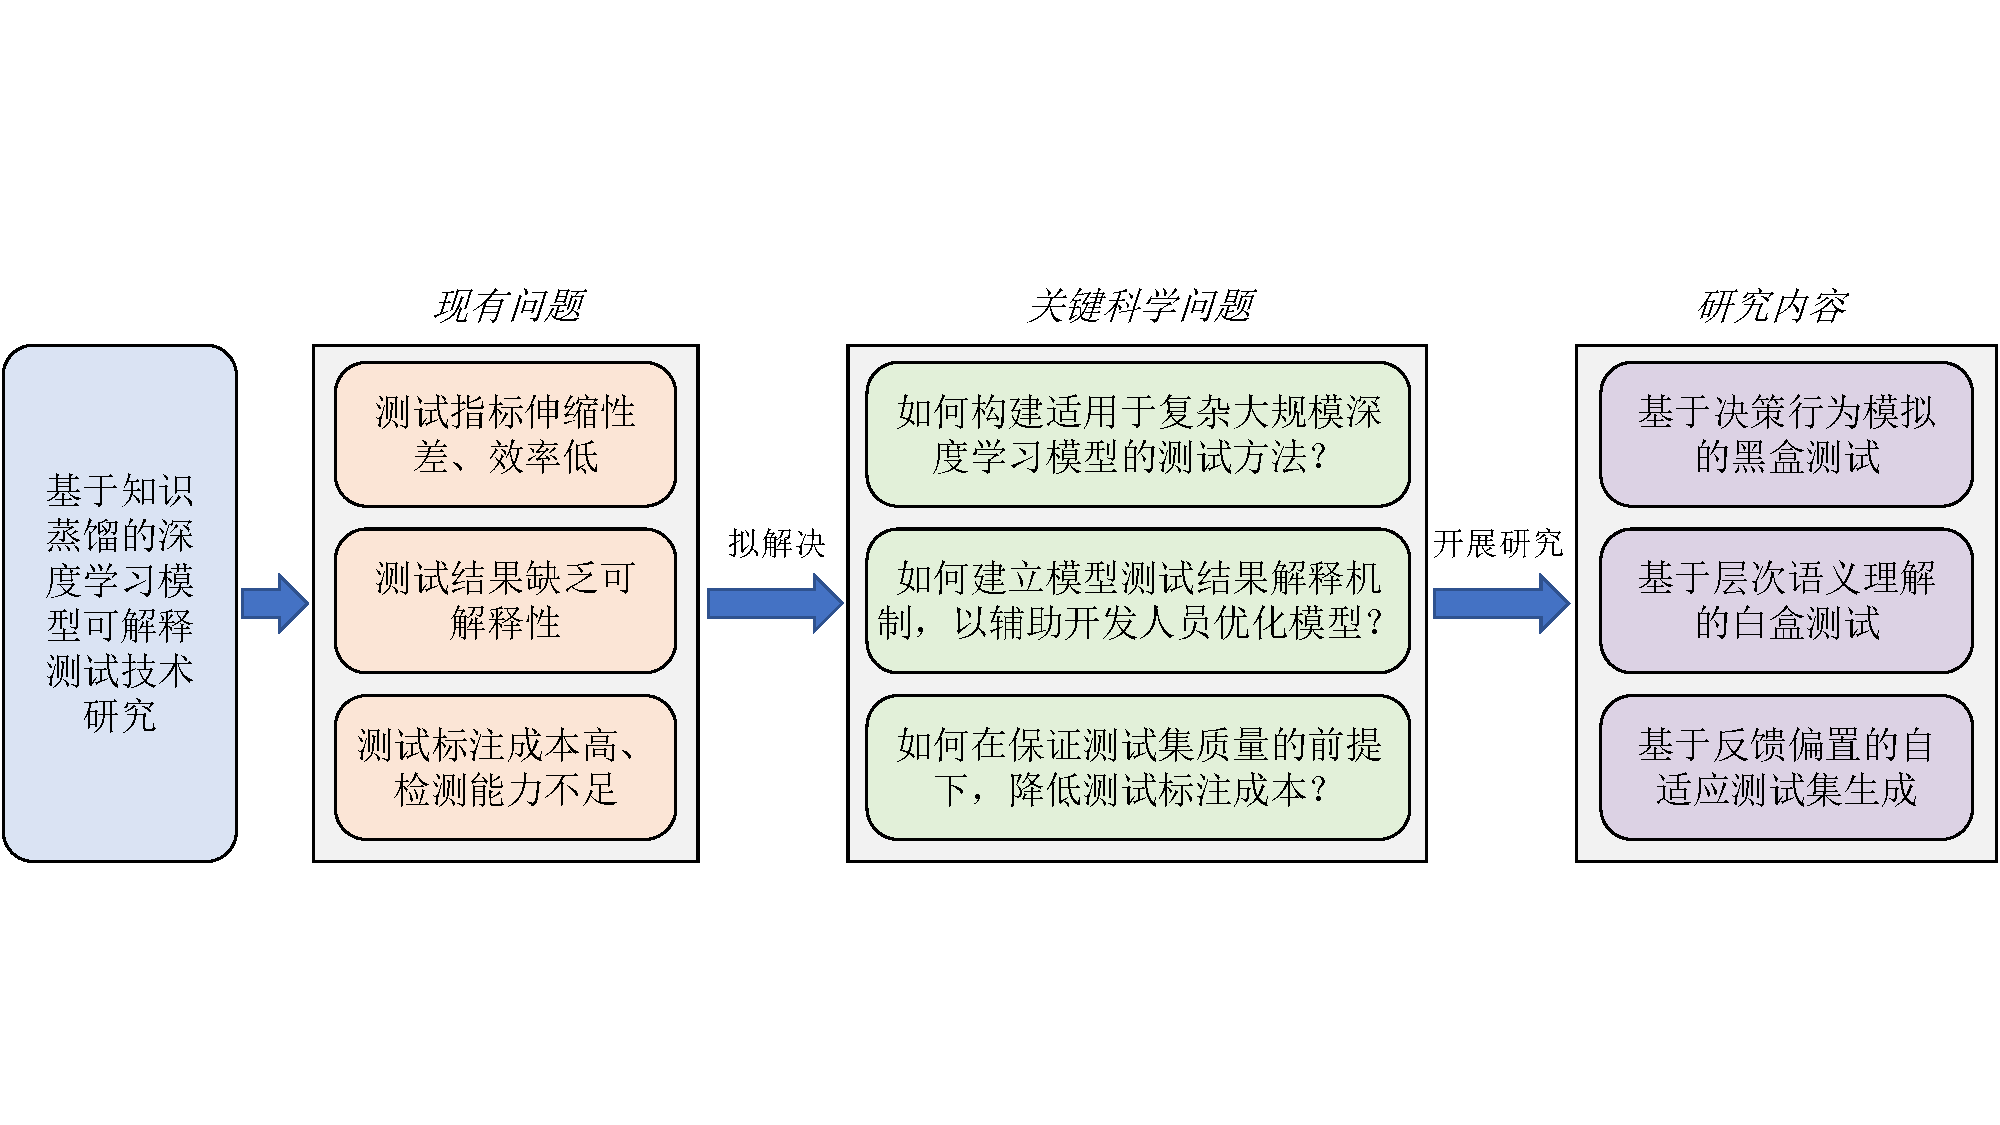
\includegraphics[width=0.95\textwidth]{ch2_framework.pdf}
        \end{center}
        \caption{挑战、科学问题和研究内容关系图}
        \label{fig:ch2:rc}
    \end{small}
\end{figure}

\begin{comment}
相比于传统机器学习模型,深度学习模型能更有力地捕捉特征之间地复杂关系以及较长时间
跨度的依赖关系,因此,本项目拟以深度学习为核心方法,结合电子医疗记录的特点,研究
电子医疗记录预测性分析关键技术,主要包括基于表现型的自动队列识别、融合医学偏差的
EMR自动插补、面向多元时间序列的特征重要性和时间关联性挖掘。各部分研究内容详细介
绍如下:
\end{comment}

\subsubsection{基于表现型的自动队列识别}

队列识别(cohort identification)通常是通过预先设定患者表现型(phenotype),然后
筛选符合该表现型的患者。表现型是指一组可以被观察到的人体器官物理或者生化的指标,
比如某种疾病、血型、身高等。电子医疗记录特征(医疗概念)维度高,特征的时间跨度差
异大,依靠医务人员人为筛选队列难以完成。利用机器学习模型实现自动队列识别具有重要
意义,是电子医疗记录分析的基础。

图~\ref{fig:ch2:ci}展示了队列识别的研究内容。给定一个电子医疗数据集,包含$N$个患
者的电子医疗记录,第$i$个患者表示为$\bm X_i = [\bm x_i^{(1)}; \bm x_i^{(2)};
\cdots; \bm x_i^{(t_i)}]$,其中$\bm x_i^{(k)}$表示患者在时间点$(k)$访问医院,
$t_i$表示第$i$个患者来医院的时间点总数。需要注意的是,在相同时刻,患者会有多条记
录(多个医疗特征),$\bm x_i^{(k)}$的维度等于全部医疗特征念集合的元素个数。对于
患者$i$而言,如果在对应的时间点有关于某个特征的记录,则向量对应的元素为记录值,
若某个特征没有观测值,则$\bm x_i^{(k)}$对应的元素没有值,记为\textit{NA}。预设的
表现型$\bm y_i$即为本问题的标签,表现型通常具有组合性,即$\bm y_i$包含多个预定的
筛选条件,记为$\bm y_i \in \{0, 1\}^c$,即$\bm y_i$是一个$c$维向量,每一维对应一
个队列筛选的条件。队列识别即给定患者的电子医疗记录$\bm X_i$,判断该患者是否满足
预定的表现型$\bm y_i$。\textbf{特征的高维性和表现型的组合性为队列识别带来了巨大
的挑战,本项目拟研究可处理长时间依赖的层次表示模型,在不损失电子医疗记录语义的情
况下,自动学习患者的抽象表示}。

\begin{figure}
    \begin{small}
        \begin{center}
            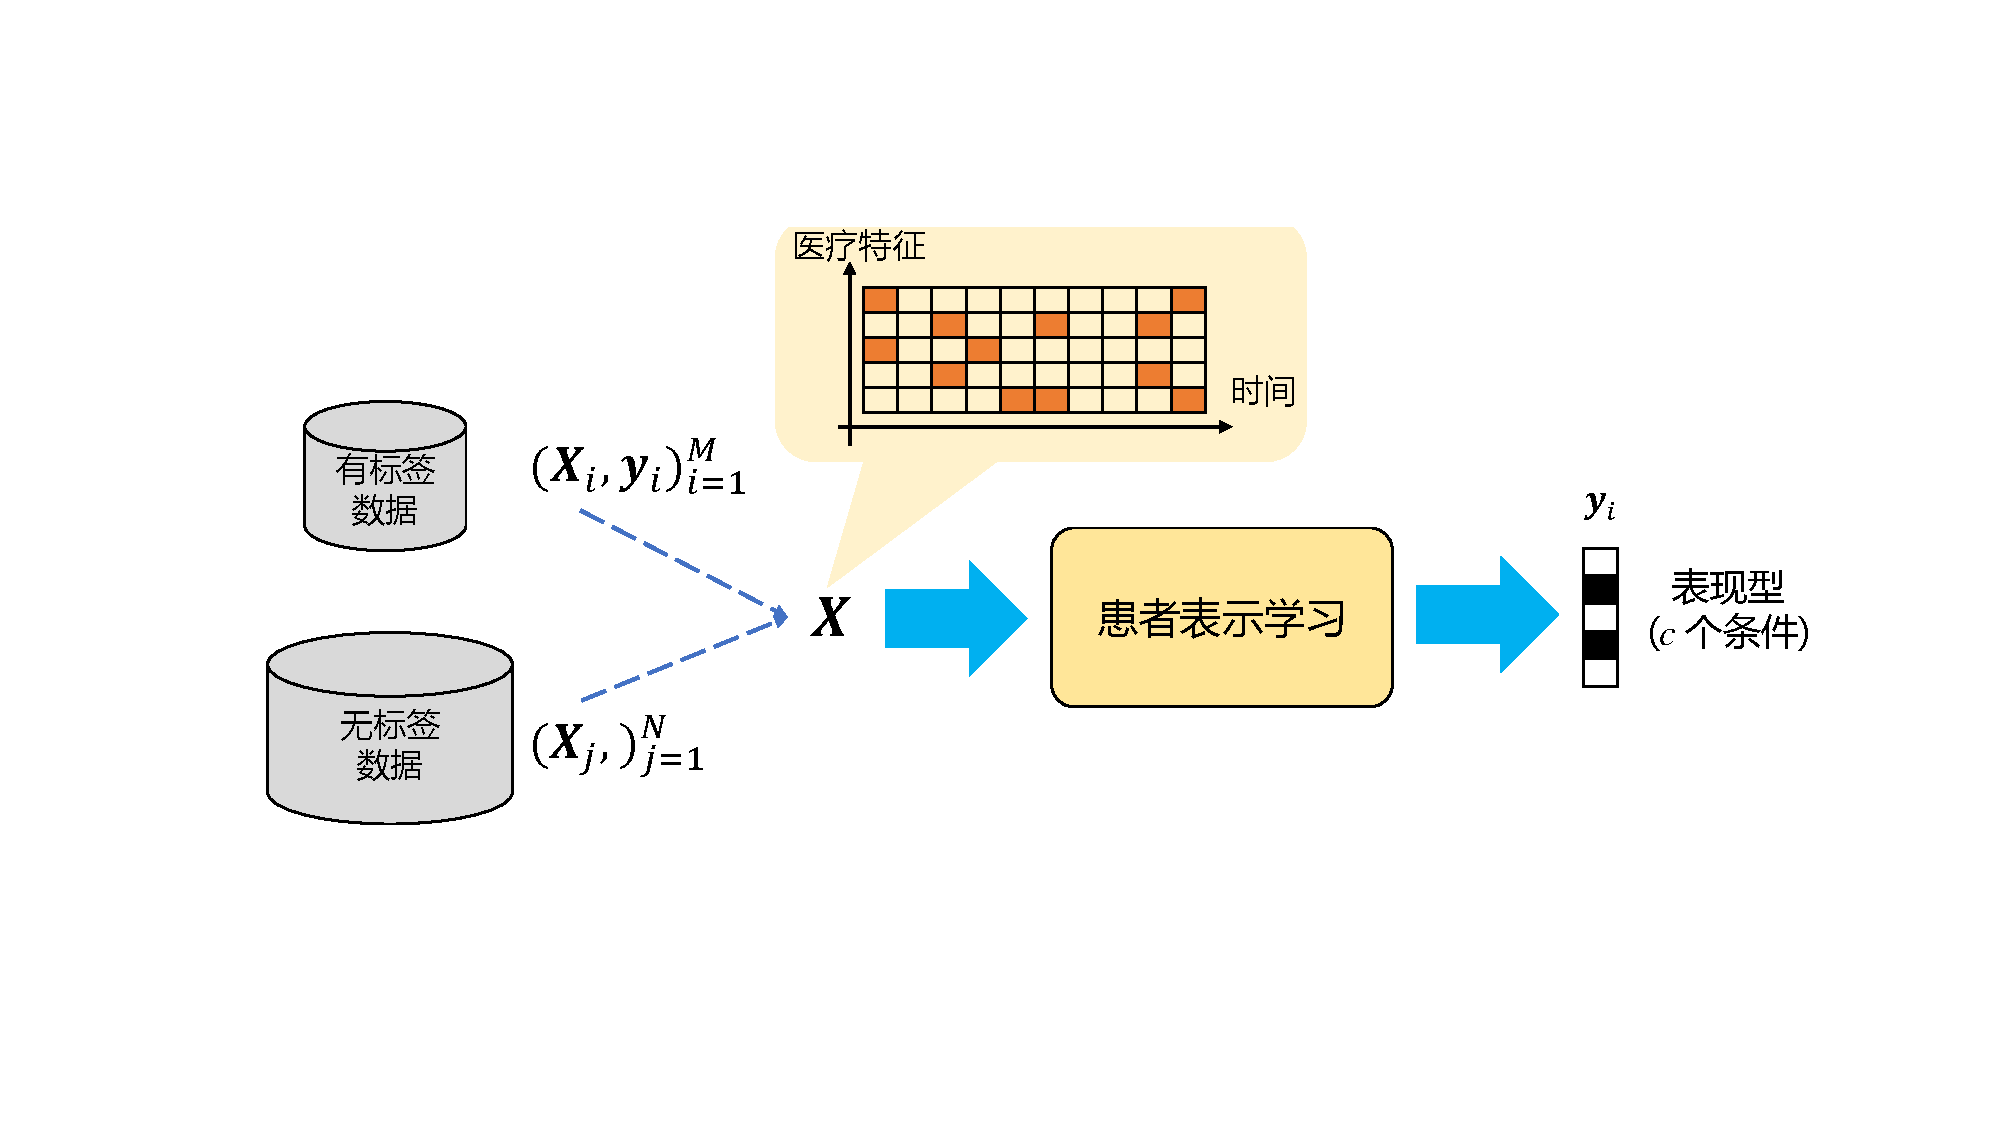
\includegraphics[width=0.8\textwidth]{ch2CI}
        \end{center}
        \caption{队列识别研究内容}
        \label{fig:ch2:ci}
    \end{small}
\end{figure}

其次,队列识别任务标注成本太高,通常难以获得大规模标注数据。一般情况下,假设在给
定的电子医疗记录中,$M$个样本是已经请专家标注的,记为$\mathcal L \triangleq (\bm
X_i, \bm y_i)_{i=1}^M$,而剩下的$N$个样本为未标注样本:$\mathcal U \triangleq
(\bm X_j,)_{j=1}^N$,未标注数据远多于标注数据,即$M \ll N$。现有方法可分为两类:
一是只是用标注样本建模,由于没有利用未标注样本,其准确性和泛化能力较差;二是利用
半监督方式训练,但在半监督模型中,标注数据和未标注数据是分开训练的,模型训练结果
容易受未标注数据影响而学习到有偏的患者表示。\textbf{本项目拟研究在仅有少量标注数
据的条件下,如何有效结合未标注数据进行训练,提升电子医疗记录表示学习效果,提高队
列识别的准确率。}。

\subsubsection{融合医学偏差的EMR自动插补}

患者就医时间不规律,且不同医疗特征的记录频率也差别很大,导致电子医疗记录具有时间
不规则性和稀疏性的特点,为电子医疗记录分析带来了新的挑战。本项目拟研究通用的电子
医疗记录插补方法,对电子医疗记录进行预处理,使其在时间维度上更为规则,降低后续分
析的模型复杂度。

\begin{figure}
    \begin{small}
        \begin{center}
            \includegraphics[width=0.85\textwidth]{ch2imputation.pdf}
        \end{center}
        \caption{EMR插补研究内容}
        \label{fig:ch2:imputation}
    \end{small}
\end{figure}

图~\ref{fig:ch2:imputation}举例说明了本项目电子医疗记录插补的研究内容。给定电子
医疗记录$\bm X$,若电子医疗记录一共有$d$个特征,$t$个时间点,则$\bm X \in
\mathbb{R}^{d\times t}$。本项目拟构建机器学习模型推断$\bm X$中的部分缺失值,即图
中\textit{NA}所在的位置,最终得到数值完整的电子医疗记录,如图中$\bm X_{ipt}$所
示。

现有工作利用RNN、Transformer~\citess{vaswani2017attention}和它们的变种针对时间维
度进行建模,但现有工作没有考虑电子医疗记录产生过程引入的医学偏差,导致部分插补不
够准确。电子医疗记录不能直接反映患者的健康状态,因为这些记录的产生除了源自患者的
健康状态,还蕴含着患者与电子病历系统的“交互”过程,通常会引入系统偏差。医学研究表
明~\citess{agniel2018biases},\textbf{医学偏差不应被看作数据质量问题或者噪声,而
是一种数据细分的信号},如:肾衰竭的患者更可能在晚上10点到早上6点之间化验肌酐;重
病患者做检查更加频繁等。记录产生的时间可以反映特征记录的过程,是模型理解医学偏差
的重要途经。如图~\ref{fig:ch2:imputation}所示,本项目拟结合患者的缺失标记矩阵和
就医时间学习特征缺失规律,在EMR插补模型中引入医学偏差。若时间$(k)$时患者第$i$个
特征被记录下来,则图中缺失标记矩阵$\bm M$的对应取值$m_i^{(k)}=1$,若没观察到,则
$m_i^{(k)}=0$,缺失矩阵和记录时间完整地反映了医疗特征的缺失规律,可用于理解医学
偏差。\textbf{本项目拟研究如何利用缺失矩阵和记录时间为EMR插补模型引入医学偏差,
以实现隐式的数据细分,提升EMR插补的准确性和合理性}。

\subsubsection{结合特征重要性和时间关联性的可解释预测模型}

如图~\ref{fig:ch2:interpretability}所示,电子医疗记录除了包含随时间变化的医疗特
征,还会包含患者的人口统计学特征,如性别、种族等,这些特征虽然是静态不变的,但对
预测患者病情发展也非常重要,所以\textbf{在构建预测模型时,首先应该研究如何将患者
的静态特征和动态特征分别建模,以及如何融合两组特征进行分析}。

\begin{figure}
    \begin{small}
        \begin{center}
            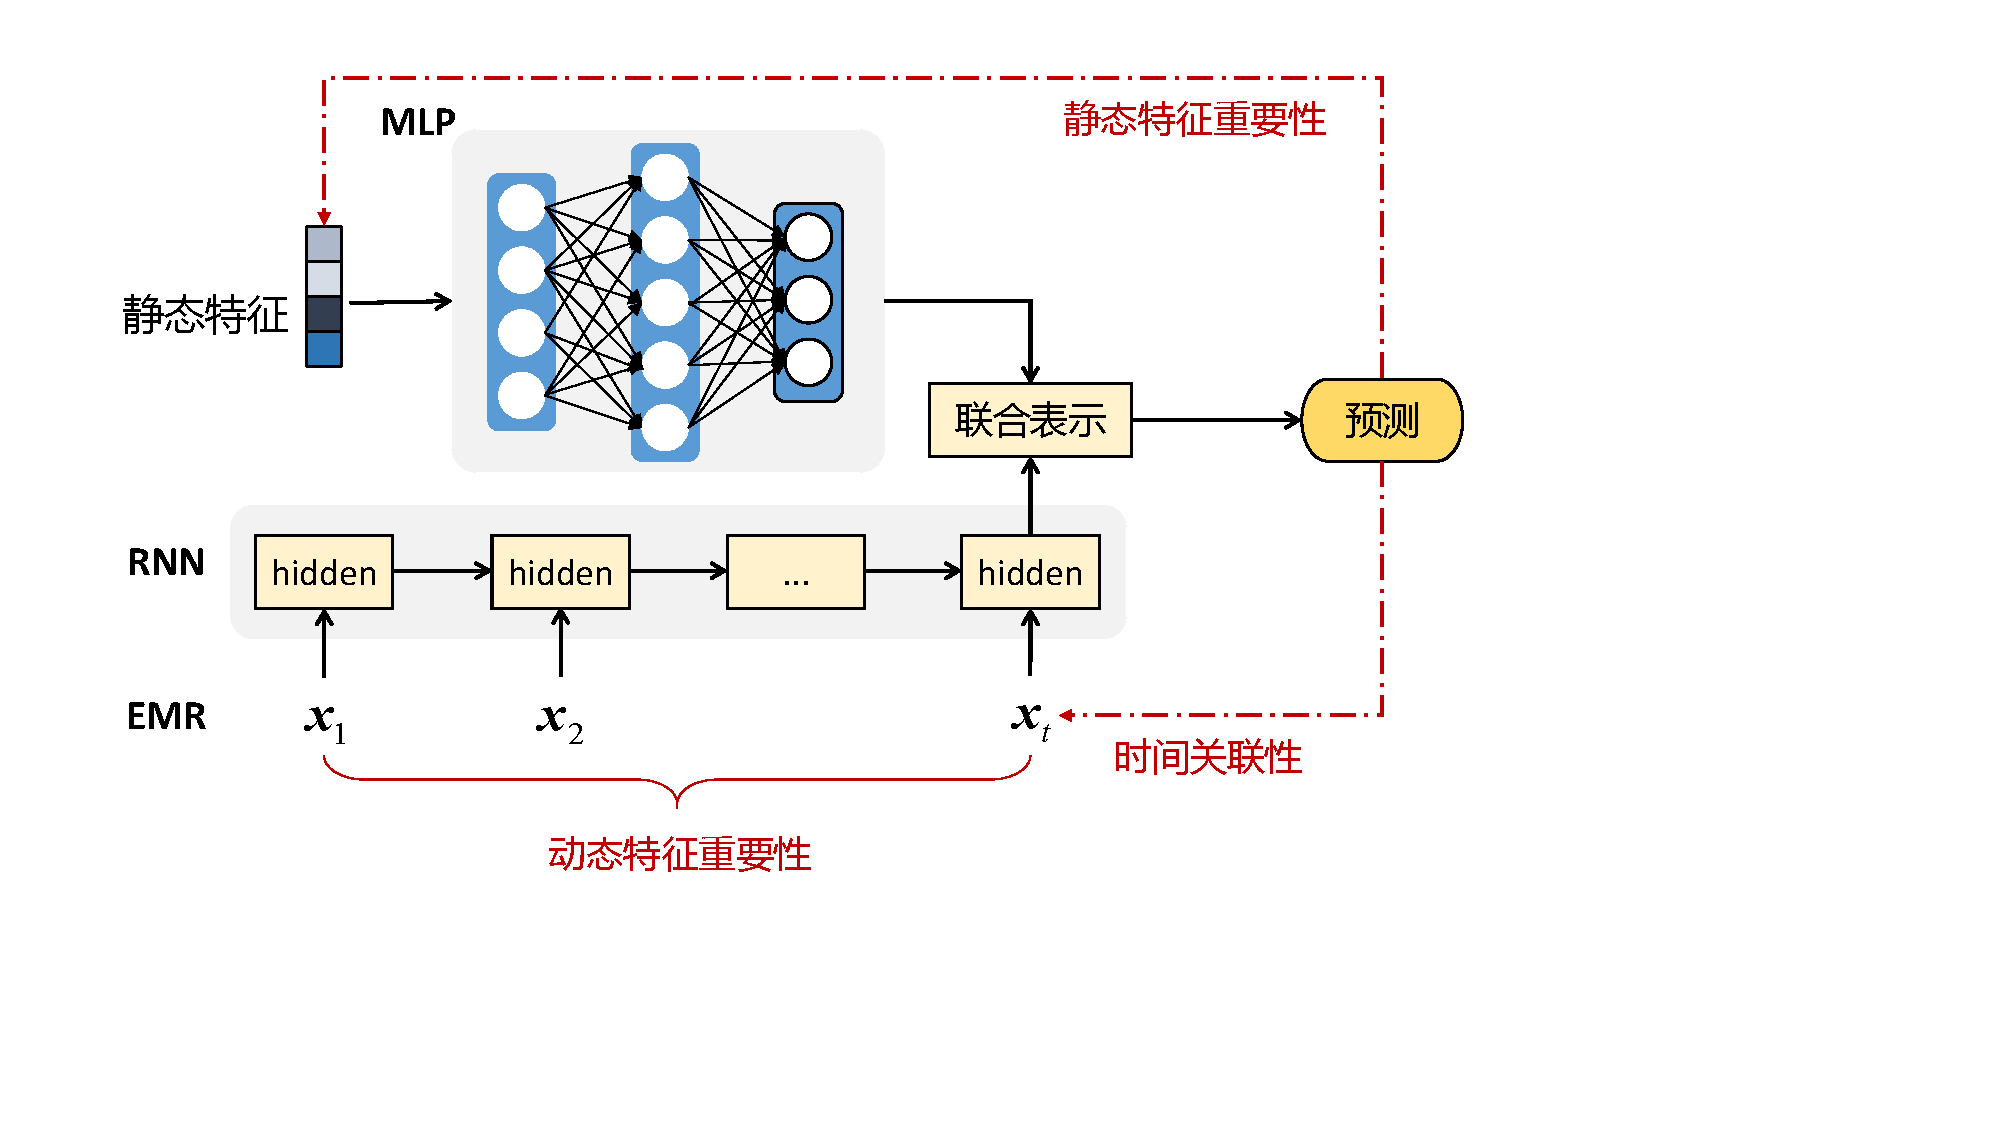
\includegraphics[width=0.75\textwidth]{ch2Interpretability.pdf}
        \end{center}
        \caption{可解释预测模型研究内容}
        \label{fig:ch2:interpretability}
    \end{small}
\end{figure}

模型的临床应用需要提供对模型和预测结果的解释,因此,预测模型的可解释性是本项目另
一个重要的研究内容。目前用于电子医疗记录分析的可解释方法可分为两类:第一类研究在
预测模型建模时没有考虑其解释性,但利用后解释(post-interpretable)模型来解释预测
结果,这类方法具有两个缺点,一是后解释模型把任何预测模型当作黑盒,依然无法让医生
了解模型真实的决策过程,只能提供预测结果的可靠程度,二是随着就诊数据的变化,需要
重新训练预测模型和后解释模型,带来了额外开销;第二类研究在预测模型中实现可解释
性,在完成预测的同时,也能为预测结果提供可解释的依据,这类方法尝试在预测准确性和
可解释性两方面找到一种平衡,通常在模型实现可解释性时,其准确率会有所下降。

本项目拟在预测模型中考虑可解释性,现有工作缺少对静态特征和动态特征的统一比较,无
法得到模型的全局可解释性。静态特征通常用浅层全连接层建模,本项目拟采用逐层相关性
传播~\citess{bach2015pixel}分析静态特征与预测结果的关系。而对动态特征,本项目拟
采用RNN模型进行建模,但由于RNN复用隐含层,其针对多维特征的可解释特别差,一方面,
隐含层是由所有特征经过多步计算得到的,无法从隐含层解耦出每个特征对预测结果的贡
献;另一方面,RNN中最后的隐含层是由多步计算得到,其时间信息也无法逆向得到,阻碍
了特征出现时间的分析。所以动态特征可解释性研究的重点在于分析高维的动态特征与预测
目标的关系。\textbf{本项目通过对RNN隐含层解耦,挖掘动态特征重要性和时间关联性,
并统一比较动态特征和静态特征的贡献,实现模型的全局解释,且可回溯样本预测结果,为
医务人员提供全面的模型解释}。

\subsubsection{临床预测性任务}

\textbf{本项目拟将研究成果应用于具体的临床预测性任务,以验证其有效性,同时,通过
和临床医生的合作,提高研究质量,加速研究成果应用}。具体而言,本项目拟将研究成果
应用于慢性肾脏病进展预测和急诊科感染性休克预警,并通过和医生的交流,保证项目研究
内容具有实际应用价值。

\begin{itemize}
    \item  \textbf{与北京大学医疗健康大数据国家研究院合作,预测DKD慢性肾病患者的
    病情发展情况},提醒医生及时进行临床干预。
    \item  利用机器学习手段预测病人状态对降低ICU感染性休克的病发率和死亡率具有重
    要意义。\textbf{本项目拟基于MIMIC-III~\citess{johnson2016mimic},利用项目研
    究成果实现ICU患者感染性休克预警系统},验证项目研究成果的有效性。
\end{itemize}


\subsection{研究目标}\label{ch2target}

本项目从医疗卫生行业和人工智能结合的实际需求出发,针对队列识别泛化能力差、EMR插
补准确率低、以及预测模型可解释性匮乏等问题,研究队列识别、EMR插补和可解释预测模
型等问题,并将相关研究成果应用实际临床数据,检验本项目的研究成果在电子医疗记录预
测性分析中的应用效果,推动电子医疗记录分析的研究进展。

具体研究目标包括:

\textbf{在技术方面},本项目拟在以下四方面实现技术突破: (a) 提出基于表现型的队列
识别方法,充分利用已标注和未标注数据,提高队列识别模型的准确性和表示学习的泛化能
力;(b) 提出融合医学偏差的EMR自动插补方法,实现数据预处理,通过合理引入医学偏
差,提高EMR插补的准确性;(c) 提出可解释预测模型,在进行预测的同时,可以从模型中
得到与预测目标相关的特征和时间点;(d) 将本项目的研究成果应用于DKD患者病情进展预
测和重症监护室患者感染性休克预测。

\textbf{在成果形式方面},本项目力争在国内外高水平期刊、会议上发表论文8篇以上,全
部被SCI/EI检索,其中有重要影响的论文4篇以上;申请专利2项。

\textbf{在人才培养方面},通过本项目研究,培养深度学习、电子医疗记录分析、可解释人工智能等交叉领域的青年人才,拟培养研究生3-4人。

\subsection{拟解决的关键科学问题}

基于上述研究目标和研究内容,本项目拟在以下几个关键理论和技术问题上有所突破:

\subsubsection{在弱监督条件下构建泛化性强的患者层次表示,实现自动队列识别}

从海量、高维的电子医疗记录中识别研究队列是电子医疗记录分析的基础,由于电子医疗记
录的高维性和表现型的组合性,依靠医务人员人力筛选和标注所有符合预定表现型的队列数
据不具有可操作性。患者的表现型表示可以更准确地对应预定义表现型,提高队列识别准确
度,但仅基于少量队列标签的EMR数据集不足以让模型学习到好的数据分布,同时,传统半
监督方法在标注数据和未标注数据上分别训练,模型的训练更容易被未标注数据影响。因
此,如何合理利用大量未标注数据辅助建模,构建泛化性强的患者层次表示,实现电子医疗
记录的队列识别是本项目拟解决一个关键科学问题。

\subsubsection{建立医学偏差和缺失矩阵的对应关系,并将其融入电子医疗记录插补中}

电子医疗记录具有时间不规则性,直接在电子医疗记录上建模和训练难以得到较好的结果,
训练得到的模型通常容易过拟合,泛化性较差。在构建预测模型之前对电子医疗记录进行插
补具有重要意义,可以降低预测模型复杂度和训练难度。现有方法忽略了电子医疗记录中固
有的医学偏差,将其中的缺失值当作完全随机缺失对待,其插补结果不够准确。医学偏差并
不是数据质量问题或者噪声,反而对充分理解电子医疗记录非常重要。如何建立医学偏差和
记录缺失的对应关系,并将其融合到电子医疗记录插补中是本项目构建通用电子医疗记录处
理框架要解决的一个关键科学问题。

\subsubsection{融合特征重要性和时间关联性,建立电子医疗记录可解释分析模型}

模型的可解释性对医学领域的预测性分析至关重要,决定了模型是否能应用于临床实践。电
子医疗记录(动态特征)是一种特殊的多元时序数据,通常采用RNN模型建模,但在RNN学习
过程中,多个特征在不同时间点的取值都被糅合在RNN的隐含层中,无法总结得到特征对于
模型的意义,也无法计算出某条记录和预测结果的相关性。因此,如何融合特征重要性和时
间关联性,构建可解释预测模型,支持模型的全局解释和预测结果的回溯,也是本项目拟解
决的一个关键科学问题。